\section{Test Setup per Research Question (NEW: since last update, NEW, NEW: Since last update i have created the aboce mentioned webapp so i will next adapt the test setups!)}
\label{sec:test-setup-per-research-question}
    I will now propose one test setup per research qustion and then try out each test setup. One very important change to the initial testing setup described in Figure \ref{fig:initial_network_layout} is that i will be using my PC and its 2.5 GbE NIC to generate load for the devices under test.
    \subsection{How does power consumption change with the number of active Ethernet ports? Is there a measurable difference between 100 Mbps and 1 Gbps connections, in different load scenarios?}
    \label{sec:test-setup-rq1}
    \subsubsection{Test Setup}
    To investigate power consumption with varying numbers of active Ethernet ports and different connection speeds, we will use the following setup:

    \begin{figure}[H]
        \centering
        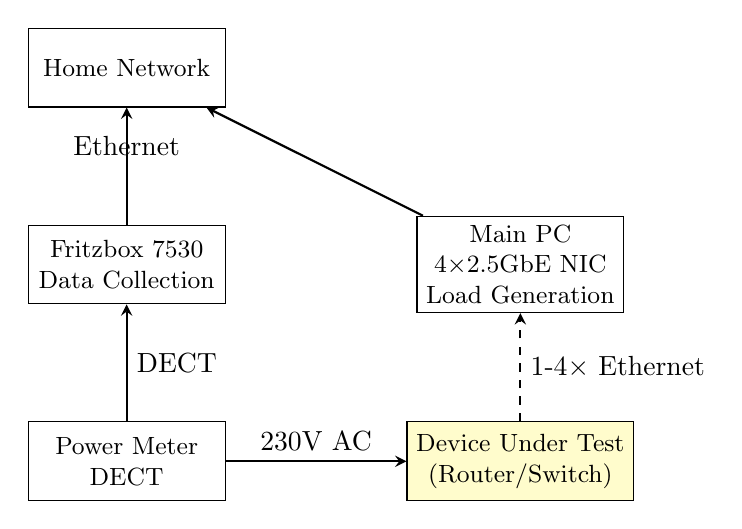
\begin{tikzpicture}[
            box/.style={rectangle, draw, minimum width=2.5cm, minimum height=1cm, text centered, font=\small, align=center},
            arrow/.style={->, >=stealth, thick}
        ]
            % Power Meter
            \node[box] (meter) at (0,0) {Power Meter\\DECT};
            
            % Fritzbox
            \node[box] (fritzbox) at (0,2.5) {Fritzbox 7530\\Data Collection};
            
            % Device Under Test
            \node[box, fill=yellow!20] (dut) at (5,0) {Device Under Test\\(Router/Switch)};
            
            % Main PC
            \node[box] (pc) at (5,2.5) {Main PC\\4$\times$2.5GbE NIC\\Load Generation};
            
            % Home Network
            \node[box] (network) at (0,5) {Home Network};
            
            % Connections
            \draw[arrow] (meter) -- node[right] {DECT} (fritzbox);
            \draw[arrow] (fritzbox) -- node[above] {Ethernet} (network);
            \draw[arrow] (meter) -- node[above] {230V AC} (dut);
            \draw[arrow, dashed] (dut) -- node[right] {1-4$\times$ Ethernet} (pc);
            \draw[arrow] (pc) -- (network);
            
        \end{tikzpicture}
        \caption{Test Setup for Ethernet Port and Speed Analysis}
        \label{fig:test_setup_rq1}
    \end{figure}

    \textbf{Test Procedure:}
    \begin{enumerate}
        \item Connect the device under test to the power meter
        \item Connect 1, 2, 3, and 4 Ethernet cables from the main PC's NIC to the device under test
        \item For each cable count, test with:
        \begin{itemize}
            \item Idle load (no traffic)
            \item 50\% load using iperf3
            \item 100\% load using iperf3
        \end{itemize}
        \item Force connections to 100 Mbps and repeat tests
        \item Force connections to 1 Gbps and repeat tests
        \item Record power consumption data via Fritzbox TR064 API
    \end{enumerate}

    \subsection{How does power consumption scale with network load (idle, 50\%, 100\% utilization of bandwidth)?}
    \label{sec:test-setup-rq2}

    \subsubsection{Test Setup}
    \begin{figure}[H]
        \centering
        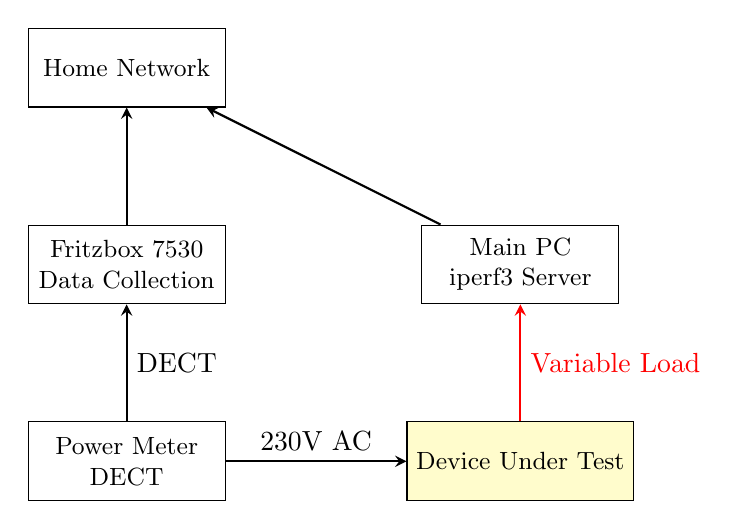
\begin{tikzpicture}[
            box/.style={rectangle, draw, minimum width=2.5cm, minimum height=1cm, text centered, font=\small, align=center},
            arrow/.style={->, >=stealth, thick}
        ]
            \node[box] (meter) at (0,0) {Power Meter\\DECT};
            \node[box] (fritzbox) at (0,2.5) {Fritzbox 7530\\Data Collection};
            \node[box, fill=yellow!20] (dut) at (5,0) {Device Under Test};
            \node[box] (pc) at (5,2.5) {Main PC\\iperf3 Server};
            \node[box] (network) at (0,5) {Home Network};
            
            \draw[arrow] (meter) -- node[right] {DECT} (fritzbox);
            \draw[arrow] (fritzbox) -- (network);
            \draw[arrow] (meter) -- node[above] {230V AC} (dut);
            \draw[arrow, thick, red] (dut) -- node[right] {Variable Load} (pc);
            \draw[arrow] (pc) -- (network);
        \end{tikzpicture}
        \caption{Test Setup for Network Load Scaling Analysis}
        \label{fig:test_setup_rq2}
    \end{figure}

    \textbf{Test Procedure:}
    \begin{enumerate}
        \item Configure iperf3 server on main PC
        \item For each device under test:
        \begin{itemize}
            \item Measure idle power consumption (5 minutes)
            \item Run iperf3 at 50\% bandwidth limit (10 minutes)
            \item Run iperf3 at 100\% bandwidth (10 minutes)
        \end{itemize}
        \item Test devices: Fritzbox 7530, Asus RT-AX68U, Alcatel HH40V, Huawei EG8245W5-8T
    \end{enumerate}

    \subsection{Which equipment is suitable for continuous operation and which devices have high idle consumption that makes them candidates for automated shutdown during off-peak hours?}
    \label{sec:test-setup-rq3}

    \subsubsection{Test Setup}
    This research question uses the same physical setup as RQ2, but focuses on long-term idle measurements.

    \textbf{Test Procedure:}
    \begin{enumerate}
        \item Measure 24-hour idle power consumption for each device
        \item Record power consumption during typical usage patterns
        \item Calculate daily energy cost at current electricity rates
        \item Identify devices with standby power $>$ 2W as shutdown candidates
    \end{enumerate}

    \subsection{How does power consumption per client differ between Ethernet and Wi-Fi connections?}
    \label{sec:test-setup-rq4}

    \subsubsection{Test Setup}
    \begin{figure}[H]
        \centering
        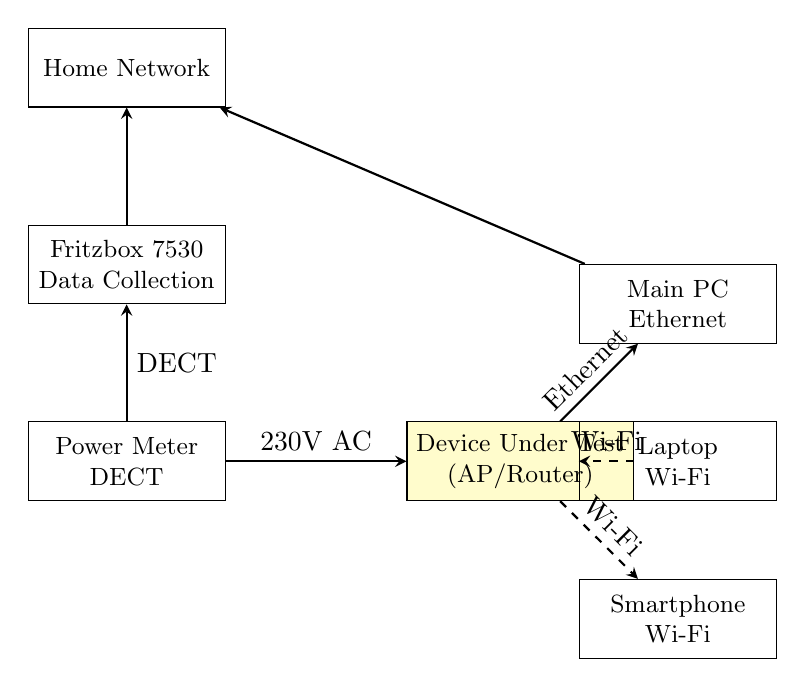
\begin{tikzpicture}[
            box/.style={rectangle, draw, minimum width=2.5cm, minimum height=1cm, text centered, font=\small, align=center},
            arrow/.style={->, >=stealth, thick}
        ]
            \node[box] (meter) at (0,0) {Power Meter\\DECT};
            \node[box] (fritzbox) at (0,2.5) {Fritzbox 7530\\Data Collection};
            \node[box, fill=yellow!20] (dut) at (5,0) {Device Under Test\\(AP/Router)};
            \node[box] (pc1) at (7,2) {Main PC\\Ethernet};
            \node[box] (pc2) at (7,0) {Laptop\\Wi-Fi};
            \node[box] (phone) at (7,-2) {Smartphone\\Wi-Fi};
            \node[box] (network) at (0,5) {Home Network};
            
            \draw[arrow] (meter) -- node[right] {DECT} (fritzbox);
            \draw[arrow] (fritzbox) -- (network);
            \draw[arrow] (meter) -- node[above] {230V AC} (dut);
            \draw[arrow] (dut) -- node[above,sloped] {Ethernet} (pc1);
            \draw[arrow, dashed] (dut) -- node[above,sloped] {Wi-Fi} (pc2);
            \draw[arrow, dashed] (dut) -- node[above,sloped] {Wi-Fi} (phone);
            \draw[arrow] (pc1) -- (network);
        \end{tikzpicture}
        \caption{Test Setup for Ethernet vs Wi-Fi Client Analysis}
        \label{fig:test_setup_rq4}
    \end{figure}

    \textbf{Test Procedure:}
    \begin{enumerate}
        \item Baseline: measure power with no clients connected
        \item Connect 1-4 clients via Ethernet, measure power consumption
        \item Connect 1-4 clients via Wi-Fi (2.4GHz), measure power consumption
        \item Connect 1-4 clients via Wi-Fi (5GHz), measure power consumption
        \item Generate identical network load across all scenarios using iperf3
        \item Calculate power consumption per client for each connection type
    \end{enumerate}

    \subsection{What is the actual impact of power-saving modes on overall power consumption?}
    \label{sec:test-setup-rq5}

    \subsubsection{Test Setup}
    Uses the same setup as RQ2, comparing devices with power-saving features enabled vs disabled.

    \textbf{Test Procedure:}
    \begin{enumerate}
        \item For devices with Energy Efficient Ethernet (EEE):
        \begin{itemize}
            \item Measure idle power with EEE enabled
            \item Measure idle power with EEE disabled
            \item Measure under load with EEE enabled/disabled
        \end{itemize}
        \item For devices with Wi-Fi power-saving modes:
        \begin{itemize}
            \item Test with various power-saving settings
            \item Measure impact on both device and client power consumption
        \end{itemize}
    \end{enumerate}

    \subsection{Does the type of connected device or wireless signal strength affect power consumption?}
    \label{sec:test-setup-rq6}

    \subsubsection{Test Setup}
    \begin{figure}[H]
        \centering
        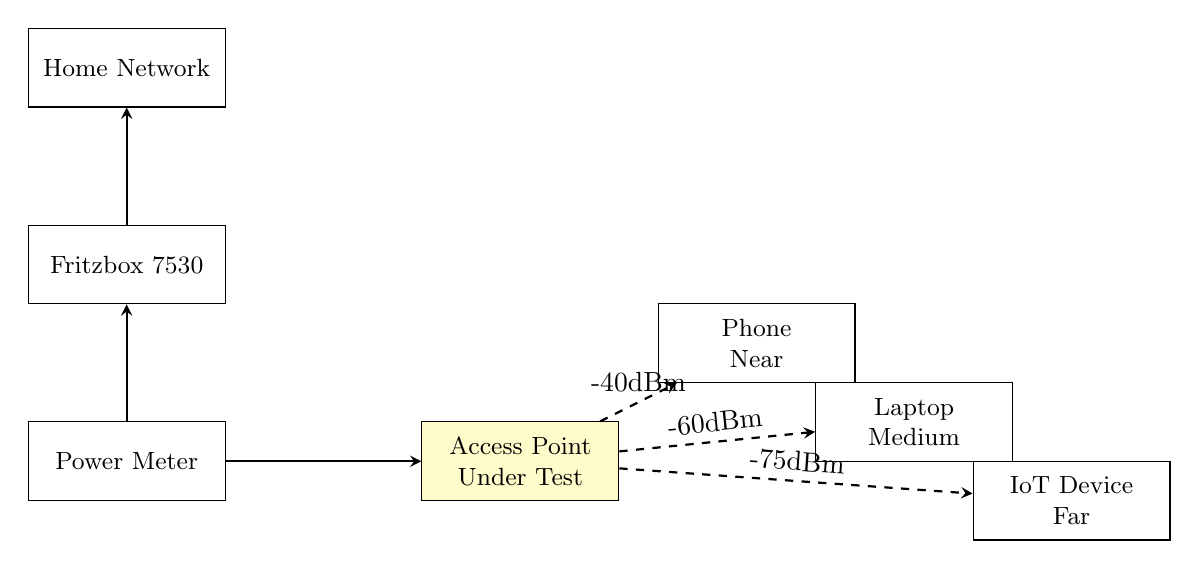
\begin{tikzpicture}[
            box/.style={rectangle, draw, minimum width=2.5cm, minimum height=1cm, text centered, font=\small, align=center},
            arrow/.style={->, >=stealth, thick}
        ]
            \node[box] (meter) at (0,0) {Power Meter};
            \node[box] (fritzbox) at (0,2.5) {Fritzbox 7530};
            \node[box, fill=yellow!20] (ap) at (5,0) {Access Point\\Under Test};
            \node[box] (d1) at (8,1.5) {Phone\\Near};
            \node[box] (d2) at (10,0.5) {Laptop\\Medium};
            \node[box] (d3) at (12,-0.5) {IoT Device\\Far};
            \node[box] (network) at (0,5) {Home Network};
            
            \draw[arrow] (meter) -- (fritzbox);
            \draw[arrow] (fritzbox) -- (network);
            \draw[arrow] (meter) -- (ap);
            \draw[arrow, dashed] (ap) -- node[above] {-40dBm} (d1);
            \draw[arrow, dashed] (ap) -- node[above,sloped] {-60dBm} (d2);
            \draw[arrow, dashed] (ap) -- node[above,sloped] {-75dBm} (d3);
        \end{tikzpicture}
        \caption{Test Setup for Device Type and Signal Strength Analysis}
        \label{fig:test_setup_rq6}
    \end{figure}

    \textbf{Test Procedure:}
    \begin{enumerate}
        \item Position clients at various distances: near ($<$2m), medium (5m), far (10m)
        \item Test with different device types: smartphone, laptop, IoT device
        \item Measure power consumption at each signal strength level
        \item Generate identical traffic patterns across all scenarios
    \end{enumerate}

    \subsection{Does maximum power rating correlate with real-world usage?}
    \label{sec:test-setup-rq7}

    \subsubsection{Test Setup}
    Uses the same physical setup as previous tests, but focuses on stress testing.

    \textbf{Test Procedure:}
    \begin{enumerate}
        \item Record rated maximum power from device specifications
        \item Measure power under maximum stress:
        \begin{itemize}
            \item All ports active at maximum speed
            \item Maximum Wi-Fi clients connected
            \item Maximum throughput on all interfaces simultaneously
        \end{itemize}
        \item Compare measured peak power to rated maximum
        \item Determine realistic power budget requirements
    \end{enumerate}

    \subsection{How efficient is ISP-provided equipment in bridge mode vs dedicated networking equipment?}
    \label{sec:test-setup-rq8}

    \subsubsection{Test Setup}
    \begin{figure}[H]
        \centering
        \begin{tikzpicture}[
            box/.style={rectangle, draw, minimum width=2.5cm, minimum height=1cm, text centered, font=\small, align=center},
            arrow/.style={->, >=stealth, thick}
        ]
            \node[box] (meter1) at (0,0) {Power Meter 1};
            \node[box] (meter2) at (0,-3) {Power Meter 2};
            \node[box] (fritzbox) at (-3,1.5) {Fritzbox 7530\\Data Collection};
            \node[box, fill=yellow!20] (isp) at (3,0) {Huawei\\EG8245W5-8T\\Bridge Mode};
            \node[box, fill=yellow!20] (router) at (3,-3) {Asus\\RT-AX68U\\Router};
            \node[box] (pc) at (6,-1.5) {Main PC};
            \node[box] (network) at (-3,4) {Home Network};
            
            \draw[arrow] (meter1) -- (fritzbox);
            \draw[arrow] (fritzbox) -- (network);
            \draw[arrow] (meter1) -- node[above] {230V} (isp);
            \draw[arrow] (meter2) -- node[above] {230V} (router);
            \draw[arrow] (isp) -- node[right] {WAN} (router);
            \draw[arrow] (router) -- (pc);
            
            % Alternative setup annotation
            \node[draw, dashed, fit=(isp)(router), inner sep=0.3cm, label=above:Setup B] {};
        \end{tikzpicture}
        \caption{Test Setup for ISP Equipment vs Dedicated Equipment Comparison}
        \label{fig:test_setup_rq8}
    \end{figure}

    \textbf{Test Procedure:}
    \begin{enumerate}
        \item Setup A: Huawei router in normal mode (all-in-one)
        \item Setup B: Huawei in bridge mode + Asus router
        \item Measure total power consumption of both setups
        \item Test under identical load conditions
        \item Calculate efficiency and total energy cost over 1 year
    \end{enumerate}
